\documentclass[12pt]{article}
\usepackage{amsthm,amssymb,amsfonts,amsmath,amstext,systeme}
\usepackage{graphicx,float}
\usepackage{tabularx}

\marginparwidth 0pt
\oddsidemargin -1.2 truecm
\evensidemargin  0pt 
\marginparsep 0pt
\topmargin -2.2truecm
\linespread{1}
\textheight 25.8 truecm
\textwidth 18.5 truecm
\newenvironment{remark}{\noindent{\bf Remark }}{\vspace{0mm}}
\newenvironment{remarks}{\noindent{\bf Remarks }}{\vspace{0mm}}
\newenvironment{question}{\noindent{\bf Question }}{\vspace{0mm}}
\newenvironment{questions}{\noindent{\bf Questions }}{\vspace{0mm}}
\newenvironment{note}{\noindent{\bf Note }}{\vspace{0mm}}
\newenvironment{summary}{\noindent{\bf Summary }}{\vspace{0mm}}
\newenvironment{back}{\noindent{\bf Background}}{\vspace{0mm}}
\newenvironment{conclude}{\noindent{\bf Conclusion}}{\vspace{0mm}}
\newenvironment{concludes}{\noindent{\bf Conclusions}}{\vspace{0mm}}
\newenvironment{dill}{\noindent{\bf Description of Dill's model}}{\vspace{0mm}}
\newenvironment{maths}{\noindent{\bf Mathematics needed}}{\vspace{0mm}}
\newenvironment{inst}{\noindent{\bf Instructions}}{\vspace{0mm}}
\newenvironment{notes}{\noindent{\bf Notes }}{\vspace{0mm}}
\newenvironment{theorem}{\noindent{\bf Theorem }}{\vspace{0mm}}
\newenvironment{example}{\noindent{\bf Example }}{\vspace{0mm}}
\newenvironment{examples}{\noindent{\bf Examples }}{\vspace{0mm}}
\newenvironment{topics}{\noindent{\bf Topics}}{\vspace{0mm}}
\newenvironment{outcomes}{\noindent{\bf Expected Learning Outcomes}}{\vspace{0mm}}
\newenvironment{lemma}{\noindent{\bf Lemma }}{\vspace{0mm}}
\newenvironment{solution}{\noindent{\it Solution}}{\vspace{2mm}}
\newcommand{\ds}{\displaystyle}
\newcommand{\un}{\underline}
\newcommand{\bs}{\boldsymbol}

\begin{document}

\baselineskip 18 pt
\begin{center}
	{\large \bf HKDSE MATH CORE 2021 Past Paper I}\\
	\vspace{2 mm}

\end{center}
\vspace{0.05cm}

\begin{enumerate}
	\item \textbf{HKDSE MATH CORE 2021 Past Paper I Q1}\\
	Simplify $(\alpha \beta^3)(\alpha^{-2}\beta^4)^5$ and express your answer with positive indices. \\(3 marks)	

	\item \textbf{HKDSE MATH CORE 2021 Past Paper I Q2}\\
	Make $a$ the subject of the formula $\dfrac{4 - 3a}{b} = 5$. \\(3 marks)

	\item \textbf{HKDSE MATH CORE 2021 Past Paper I Q3}\\
	Factorize
	\begin{enumerate}
		\item[(a)] $6x^2 + xy - 2y^2$,
		\item[(b)] $8x - 4y - 6x^2 - xy + 2y^2$.
	\end{enumerate}
	(3 marks)

	\item \textbf{HKDSE MATH CORE 2021 Past Paper I Q4}
	\begin{enumerate}
		\item[(a)] Find the range of values of $x$ which satisfy both $\dfrac{7(x - 2)}{5} > 3(x - 1)$ and $x + 4 \geq 0$.
		\item[(b)] How many positive integers satisfy both inequalities in (a)?
	\end{enumerate}
	(4 marks)


	\item \textbf{HKDSE MATH CORE 2021 Past Paper I Q5}\\
	The number of stickers owned by a boy is 3 times that owned by a girl. If the boy gives 20 of his stickers to the girl, then the number of stickers owned by the girl is 2 times that owned by the boy. Find the total number of stickers owned by the boy and the girl. \\(4 marks)

	\item \textbf{HKDSE MATH CORE 2021 Past Paper I Q6}\\
	The marked prive of a shirt is higher than its cost by \$80. The shirt is sold at a discount of 10\% on its marked price. After selling the shirt, the percentage profit is 30\%. Find the marked prive of the shirt. \\(4 marks)

	\item \textbf{HKDSE MATH CORE 2021 Past Paper I Q7}\\
	In a polar coordinate system, $O$ is the pole. The polar coordinates of the points $P$ and $Q$ are $(r, 80^\circ)$ and $(r, 140^\circ)$ respectively, where $r$ is a positive constant. It is given that the distance between $P$ and $Q$ is 21. Find	
	\begin{enumerate}
		\item[(a)] $\angle POQ$,
		\item[(b)] $r$,
		\item[(c)] the perimeter of $\triangle OPQ$.
	\end{enumerate}
	(4 marks)
	
	\item \textbf{HKDSE MATH CORE 2021 Past Paper I Q8}\\
	In Figure 1, $AB$ produced and $CD$ produced meet at the point $E$. It is given that $\angle CAE = \angle BDE$.
	\begin{figure}[H]
		\centering
		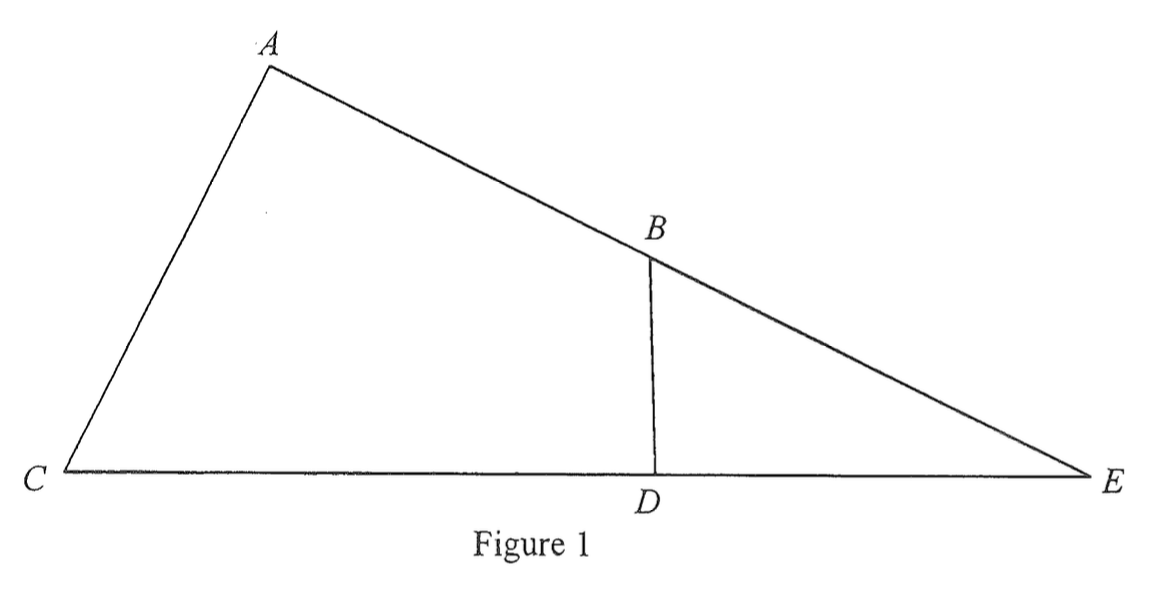
\includegraphics[width = .3\linewidth]{2021Figure1.1}
	\end{figure}
	\begin{enumerate}
		\item[(a)] Prove that $\triangle ACE \sim \triangle DBE$.
		\item[(b)] It is given that $AC = 25$ cm, $AE = 60$ cm and $BD = 15$ cm.
		\begin{enumerate}
			\item[(i)] Is $\triangle ACE$ a right-angled triangle? Explain your answer.
			\item[(ii)] Find the area of $\triangle BDE$.
		\end{enumerate}
	\end{enumerate}
	(5 marks)	
	
	\item \textbf{HKDSE MATH CORE 2021 Past Paper I Q9}\\
	The bar chart below shows the distribution of the numbers of books read by a group of students in a year.
	\begin{figure}[H]
		\centering
		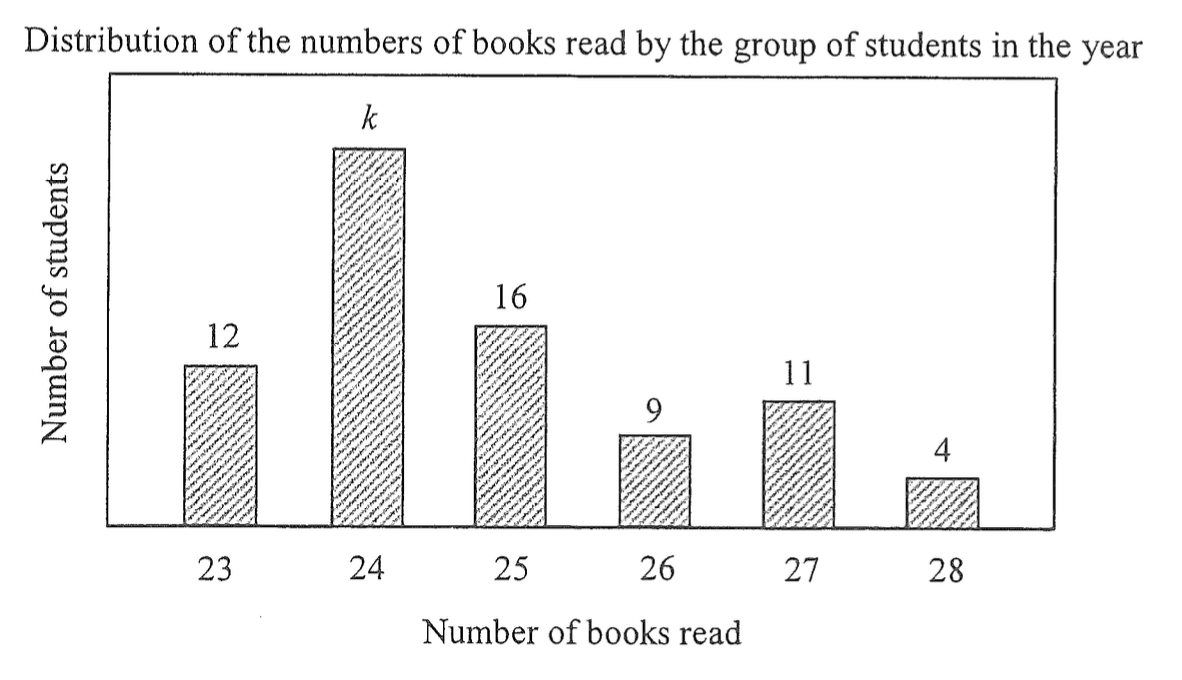
\includegraphics[width = .3\linewidth]{2021Figure1.00}
	\end{figure}
	If a student is randomly selected from the group, then the probability that the selected student reads fewer than 26 books in the year is $\dfrac{7}{10}$.
	\begin{enumerate}
		\item[(a)] Find $k$.
		\item[(b)] Write down the range the inter-quartile range and the standard deviation of the distribution.
	\end{enumerate}
	(5 marks)

	\item \textbf{HKDSE MATH CORE 2021 Past Paper I Q10}\\
	It is given that $f(x)$ is partly constant and partly varies as $(x + 4)^2$. Suppose that $f(-3) = 0$ and $f(2) = 105$.
	\begin{enumerate}
		\item[(a)] Find $f(0)$. \\(3 marks)
		\item[(b)] Denote the graph of $y = f(x) + 3$ by $G$. 
		\begin{enumerate}
			\item[(i)] Write down the $y$-intercept of $G$.
			\item[(ii)] Find the $x$-intercept of $G$.
		\end{enumerate}
		(3 marks)
	\end{enumerate}

	\item \textbf{HKDSE MATH CORE 2021 Past Paper I Q11}\\
	The table below shows the distribution of the numbers of tokens got by the group of children in a game.
	$$\begin{array}{|c|c|c|c|c|c|c|c|}
		\hline
		\text{Number of tokens got} & 1 & 2 & 3 & 4 & 5 & 6 & 7 \\
		\hline
		\text{Number of children} & 15 & 9 & 2 & 5 & 4 & 2 & 5 \\
		\hline
	\end{array}$$
	\begin{enumerate}
		\item[(a)] Find the mean of the distribution. \\(2 marks)
		\item[(b)] Are the median and the mode of the distribution equal? Explain your answer. \\(2 marks)
		\item[(c)] It $n$ more children play the game and each of them gets 5 tokens, write down
		\begin{enumerate}
			\item[(i)] the value of $n$ such taht the mean of the distribution is incrteased by 1;
			\item[(ii)] the least value of $n$ such that the median of the distribution is increased by 2;
			\item[(iii)] the greatest value of $n$ such that the mode of the distribution remains unchanged.
		\end{enumerate}
		(3 marks)
	\end{enumerate}

	\item \textbf{HKDSE MATH CORE 2021 Past Paper I Q12}\\	
	The polynomial $p(x)$ is divisible by $x - 5$. When $p(x)$ is divided by $x^2 + x + 1$, the quotient and the remainder are $2x^2 - 37$ and $cx + c - 1$ respectively, where $c$ is a constant.
	\begin{enumerate}
		\item[(a)] Find $c$. \\(3 marks)
		\item[(b)] Prove that $x+3$ is a factor of $p(x)$. \\(1 marks)
		\item[(c)] Someone claims that all the roots of the equation $p(x) = 0$ are real numbers. Is the claim correct? Explain your answer. \\(3 marks)
	\end{enumerate}

	\item \textbf{HKDSE MATH CORE 2021 Past Paper I Q13}\\
	The equation of the circle C si $x^2 +y^2 - 12x - 16y - 69 = 0$. Let $G$ be the centre of $C$. Denote the origin by $O$.
	\begin{enumerate}
		\item[(a)] Find $OG$. \\(2 marks)
		\item[(b)] Does $O$ lie inside $C$? Explain your answer. \\(1 marks)
		\item[(c)] Let $P$ be a moving point in the rectangular coordinate plane such that $OP = GP$. Denote the locus of $P$ by $\Gamma$. Suppose that cuts $C$ at the points $M$ and $N$. Find the area of the quadrilateral $OMGN$. \\(4 marks)
	\end{enumerate}

	\item \textbf{HKDSE MATH CORE 2021 Past Paper I Q14}\\
	The base radius of the solid right circular cylinder $X$ and the base radius of the solid right circular cone $Y$ are equal. The heights of $X$ and $Y$ are 20 cm and 24 cm respectively. The volume of the solid right circular cone $Z$ is equal to the sum of the volume of $X$ and the volume of $Y$. The base radius of $Z$ is equal to the base diameter of $X$. A craftsman finds that the volume of $Y$ is $800\pi$ cm$^3$.
	\begin{enumerate}
		\item[(a)] Find the base radius of $Y$. \\(2 marks)
		\item[(b)] Are $Y$ and $Z$ similar? Explain your answer. \\(3 marks)
		\item[(c)] The craftsman claims that the sum of the curved surface area of $X$ and the curved surface ares of $Y$ is greater than the curved surface area of $Z$. Do you agree? Explain your answer. \\(3 marks)
	\end{enumerate}

	\item \textbf{HKDSE MATH CORE 2021 Past Paper I Q15}\\
	A queue is randomly formed by 7 teachers and 3 students.
	\begin{enumerate}
		\item[(a)] How many different queues can be formed? \\(1 marks)
		\item[(b)] Find the probability that no students are next to each other in the queue. \\(3 marks)
	\end{enumerate}

	\item \textbf{HKDSE MATH CORE 2021 Past Paper I Q16}\\
	The straight lines $L_1$ and $L_2$ are perpendicular to each other, The $y$-intercept of $L_1$ is 3. It is given that $L_1$ and $L_2$ intersect at the point $(2,6)$. Let $R$ be the region (including the boundary) bounded by $L_1$, $L_2$ and the $x$-axis.
	\begin{enumerate}
		\item[(a)] It is given that $R$ represents the solution of a system of inequalities. Find the system of inequalities. \\(3 marks)
		\item[(b)] Find the least value of $8x - 5y$, where $(x,y)$ is a point lying in $R$. \\(2 marks)
	\end{enumerate}

	\item \textbf{HKDSE MATH CORE 2021 Past Paper I Q17}\\
	Let $A(n)$ be the $n$th term of an arithmetic sequence. It is given that $A(5) = 26$ and $A(12) = 61$.
	\begin{enumerate}
		\item[(a)] Find $A(1)$. \\(2 marks)
		\item[(b)] Suppose that $\log_2{G(n)} = A(n)$ for any positive integer $n$. Find the greatest value of $k$ such that $\log_8{\left(G(1)G(2)G(3)\cdots G(k)\right) < 999}$. \\(5 marks)
	\end{enumerate}

	\item \textbf{HKDSE MATH CORE 2021 Past Paper I Q18}
	\begin{enumerate}
		\item[(a)] A thin metal shet $ABCD$ is in the shape of a trapezium, where $AD // BC$. It is given that $AB = 45$ cm, $\angle ADC = 70^\circ$ and $\angle BAD = 50^\circ$. Find $CD$. \\(2 marks)
		\item[(b)] The metal sheet $ABCD$ described in (a) is now given. Let $E$ be a point lying on $AD$ such that $BE$ is perpendicular to $AD$. The metal sheet is folded along $BE$ such that $AE$ is perpendicular to the plane $BCDE$. Three thin triangular metal sheets are placed to this folded metal sheet to form a pyramid ( see Figure2 ). It is found that $BC = 40$ cm.
		\begin{figure}[H]
			\centering
			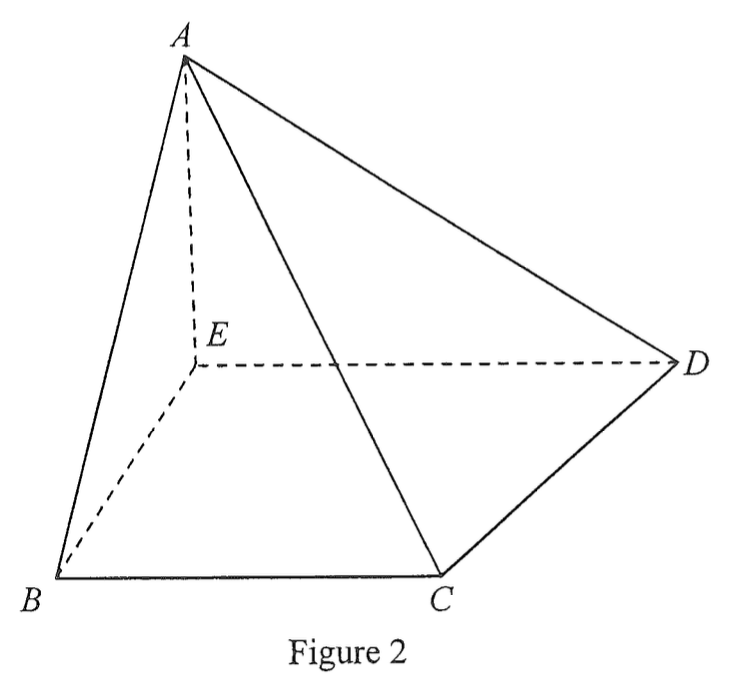
\includegraphics[width = .3\linewidth]{2021Figure1.2}
		\end{figure}
		\begin{enumerate}
			\item[(i)] Find $\angle CAD$.
			\item[(ii)] Does the angle between the plane $ACD$ and the plane $BCDE$ exceed $30^\circ$? Explain your answer.
		\end{enumerate}
		(5 marks)
	\end{enumerate}

	\item \textbf{HKDSE MATH CORE 2021 Past Paper I Q19}\\
	Let $f(x) = x^2 - 12kx -14x + 36k^2 + 89k + 53$, where $k$ is a positive constant. On the same rectangular coordinate system, denote the vertex of the graph of $y = f(x)$ and the vertex of the graph of $y  = f(14 - x)$ by $Q$ and $R$ respectively.
	\begin{enumerate}
		\item[(a)] Using the method of completing the square, express, in terms of $k$, the coordinates of $Q$. \\(2 marks)
		\item[(b)] Write down, in terms of $k$, the coordinates of $R$. \\(1 marks)
		\item[(c)] The coordinates of the point $S$ are $(7, 4 - 3k)$. Denote the inscribed circle $\triangle QRS$ by $C$.
		\begin{enumerate}
			\item[(i)] Express, in terms of $k$, the equation of the straight line which passes through $Q$ and $S$.
			\item[(ii)] Express, in terms of $k$, the equation of $C$.
			\item[(iii)] Suppose that $QS$ is the tangent to $C$ at the point $T$. Let $U$ be the centre of $C$. It is given that the coordinates of the point $V$ are $(-29, -14)$. Is it possible that $STUV$ is a rectangle? Explain your answer.
		\end{enumerate}
		(9 marks)
	\end{enumerate}


\end{enumerate}
\end{document}